\chapter{Methodology\label{ch:methods}}


\section {Dependent Variable Discussion}

The current study builds on previous literature and analyzes the factors that motivate or deter men and women to be self-employed. The Kauffman Index of Entrepreneurial Activity is used as an alternative measure for entrepreneurship, along with a comprehensive set of controls from the Current Population Survey, the National Governors' Association,  Angel Capital Association and US Bureau of Economic Analysis\footnote{The events in mind are the dot.com bubble of the early 2000s, along with the Great Recession of 2008.}. The size $N = 9,244,390$ of this constructed dataset makes it nationally representative, and its reach over the 1998-2014 period covering two great shocks on the U.S. economy, makes it temporally comprehensive. By virtue of our data and in line with existing literature, one can compute at least two different econometric models of occupational choice, with dependent variables as delineated in Parker (2004)\footnote{\cite{Parker2004}}: 
\begin{enumerate}
\item The probability $p_{entry}$ of an agent \textit{becoming self-employed} in the second survey month, given individual characteristics, occupational choice and previous work environment, as well as geographic variables and policy indicators.
\item The probability $p_{SE}$ of an agent \textit{being self-employed} at the second survey time, without the condition of wage-employment in the first survey month, with a similar set of controls, minus the ones pertaining to the transition state. 
\end{enumerate}
There are relative merits to these dependent variables, and a comprehensive discussion about their benefits and disadvantages can be found in Parker's theoretical treatment of entrepreneurship decisions\footnote{\cite[Page~26]{Parker2004}}. Several authors argue that (i) is preferable to (ii), as it separates entry and survival effects, a distinction the second model does not accomplish\footnote{\cite{EvansLeighton1989}}. This is due to the fact that the probability of being self-employed at a given time t encompasses the probability of switching into self-employment at a previous time, as well as surviving until time \textit{t}\footnote{\cite{EvansLeighton1989}}. Scholars like Wellington (2001)\footnote{\cite{Wellington2001}} on the other hand, denote that probability (i) excludes people already successfully pursuing self-employment, ignoring an inherently interesting group of observations and making for a small number of new self-employed individuals on a yearly basis. As the goal of the current paper is to estimate what drives entrepreneurship decisions, the first dependent variable, measuring the change from negative to positive self-employment status between two survey times is the most appropriate choice, allowing to capture and explain entrepreneurship as it happens. 


\section{The Probit Method}

We are interested in estimating the probability of an individual switching into self-employment under certain controls and among gender groups. In what follows, we use the Probit method to implement a series of models, with the specification that the Logit  procedure gives rise to similar results, the choice between the two depending largely on individual preference. A Probit model uses the probit link function to model the probability space for a binomial dependent variable\footnote{\cite{AldrichNelson1984}}. We assume there is an unobserved variable of interest, generated by a linear regression model of the form


\begin{dmath}
\mbox{$Y^{*}_{i} = x^{T}_i\beta + u_i = \beta_0 + \beta_1X_{i1} + \beta_2X_{i2} + ... + \beta_kX_{ik} + u_i$}
\end{dmath}
\\
in which:

$Y_i$ is a continuous variable for observation \textit{i}, that is latent or unobservable;

$x^T_i$ is, a row vector of length \textit{k} with regressor values for each observation \textit{i};

$\beta$ is a column vector of length \textit{k} containing the regression coefficients;

$x^T_i\beta$ is a term also known as the index function for observation \textit{i};

$U_i$ is the error term for observation \textit{i}, assumed to follow a normal distribution $N(0, \sigma^2)$. 


The outcomes for the binary choice problem (in our case, whether an individual opens a business or not) are represented by the indicator variable $Y_i$, mapping the unobserved dependent variable $Y^*_i$ as:

\begin{dmath}
\mbox{$Y_i = 1 \mbox{ if } Y^{*}_{i}>0$} \\
\mbox{$Y_i = 0 \mbox{ if } Y^*_i\leq 0$}
\end{dmath}

The indicator variable $Y_i$ represents the observed realizations of the binomial process, with probabilities given by:

\begin{dmath}
\mbox{$Pr(Y_i = 1) = Pr(Y^2_i > 0) = Pr (x^T_i\beta + u_i) >0 $} \\
\mbox{$Pr(Y_i = 0) = Pr(Y^2_i \leq 0) = Pr (x^T_i\beta + u_i) \leq 0 $}
\end{dmath}

Probit models represent binomial probabilities in terms of the standard normal as follows:

\begin{dmath}
\mbox{$Pr(Y_i = 1) = Pr(Y^2_i > 0) = \phi(x^T_i\beta) $} \\
\mbox{$Pr(Y_i = 0) = Pr(Y^2_i \leq 0) = 1 - \phi(x^T_i\beta) $}
\end{dmath}

The probit link function can thus be written as the inverse Gaussian cumulative distribution function, and is estimated using a standard maximum likelihood process\footnote{\cite{AldrichNelson1984}}. In a probit model, the estimate term $X\beta$ corresponds to the z-value of a normal distribution\footnote{\cite{AldrichNelson1984}}. Higher values of the estimates thus make the event more likely to happen under the given conditions. The data is expected to fit better than in a linear probability estimation, and is guaranteed to lie between 0 and 1. 

\section{Model}

We implement the probit method for three different models of entry probability, one addressing the dataset in the aggregate, and the other two focusing on the female and male samples. The first model (4.6) includes the covariate for gender, while the following two, (4.7) and (4.8) do not.


\begin{dmath}
Y^{*}_{entry} = \beta_0 + \beta_1female + \beta2ed\_years + \beta_3skill\_vers + \beta_4log\_income + \beta_5age + \beta_6age^2 + \beta_7immigr + \beta_8ed*immigr + \beta_9race + \beta_{10}mar\_stat + \beta_{11}hours\_t_0 + \beta_{12}less\_hours\_t_1 + \beta_{13}ind\_t_1 + \beta_{14}gdp\_change + \beta_{15}ed*gdp\_change + \beta_{16}unem + \beta_{17}unem\_rate + \beta_{18}gov\_party + \beta_{19}gov\_change + \beta_{20}region
\end{dmath}


\begin{dmath}
Y^{*}_{entry\_f} = \beta_0 + \beta1ed\_years + \beta_2skill\_vers + \beta_3log\_income + \beta_4age + \beta_5age^2 + \beta_6immigr + \beta_7ed*immigr + \beta_8race + \beta_{9}mar\_stat + \beta_{10}hours\_t_0 + \beta_{11}less\_hours\_t_1 + \beta_{12}ind\_t_1 + \beta_{13}gdp_change + \beta_{14}ed*gdp\_change +\beta_{15}unem + \beta_{16}unem\_rate + \beta_{17}gov\_party + \beta_{18}gov\_change + \beta_{19}region
\end{dmath}

\begin{dmath}
Y^{*}_{entry\_m} = \beta_0 + \beta_1ed\_years + \beta_2skill\_vers + \beta_3log\_income + \beta_4age + \beta_5age^2 + \beta_6immigr + \beta_7ed*immigr + \beta_8race + \beta_{9}mar\_stat + \beta_{10}hours\_t_0 + \beta_{11}less\_hours\_t_1 + \beta_{12}ind\_t_1 + \beta_{13}gdp_change + \beta_{14}ed*gdp\_change + \beta_{15}unem + \beta_{16}unem\_rate + \beta_{17}gov\_party + \beta_{18}gov\_change + \beta_{19}region
\end{dmath}

\section{Clustered Standard Errors}

We suspect observations within the same metropolitan area are correlated, as specific entrepreneurship patterns might exist at this level of granularity. To combat this problem, we implement probit models with clustered standard errors on the metropolitan area variable. A method for modeling error components, clustering maintains the assumption of zero correlation across groups, but allows for within-group correlation. We thus move from the assumption that errors are independent and identically distributed to that of observations within a city being correlated in some way, and their errors clustered.

As a result, Probit estimates remain unbiased, and the cluster-robust error estimator converges to the true standard error as the number of clusters approaches infinity, as opposed to sample size N increasing. In the context of our data, the number of clusters is high enough - we observe over 200 cities, and sufficiently balanced to allow for inference using the cluster-robust estimator. With the same logic, we also implement models with industry clustered standard errors, but choose to report the former. In doing so, we hope to see whether industries have an effect of incentivizing business formation, and whether women can penetrate male-dominated fields via self-employment. 

\section{Sparsity and Perfect Predictions}

The Kauffman Index data gives average annual rates for the transition into self-employment of about 0.5\%. This is comparatively less than the estimates of 10\% of the U.S. population being self-employed at a given time\footnote{\cite{ChatterjiGlaeserKerr2014}}, as our data captures the switch, and not the total number of business owners. This is a legitimate choice for the dependent variable, but one that given the size of our dataset and categorical nature of most explanatory variables, can create a sparsity problem. The presence of sparsity could complicate the implementation of a probit model, with the optimizer reaching a concave region where convergence is not possible. The specification of a ``difficult'' maximization problem beforehand was used to prevent this issue, allowing for the use alternative stepping algorithms in nonconcave regions\footnote{\cite{GouldPitbladoPoi2010}}.

In probit regression, another foreseeable issue is for independent variables, especially when categorical in nature, to perfectly predict one outcome or the other. For our data, industry can become a perfect predictor when used as a categorical variable, with the possibility that for a given \textit{i},

\begin{dmath}
Pr(Y = 0 | Ind_i = 1) = 1
\end{dmath}

This means that the probit coefficient on x must be minus infinity with a corresponding infinite standard error, an improbable estimation. One-way causations of this type were reported and the industry categorical variable \textit{i} eliminated from the regression model\footnote{\cite{GouldPitbladoPoi2010}}. 

\section{Evaluation of Results}

In the Probit model, one unit change in X translates to a $\beta$ change in the z-score of Y\footnote{\cite{AldrichNelson1984}}. In interpreting this result, a positive coefficient on $X_i$ translates to an increase in the predicted probability of $Y_i$. A negative coefficient means the predicted probability of $Y_i$ decreases with an increase in $X_i$\footnote{\cite{AldrichNelson1984}}. Probit p-values show the significance of a parameter, this test statistic following a standard normal distribution. As an equivalent to the coefficient of determination found in OLS regression, Probit computes the McFadden's pseudo R-squared. The total sum of squares is equivalent to the log likelihood of the intercept model, while the residual sum of squares is the log likelihood of the full model. Although caution must be employed in the evaluation of results, this approach is in line with the R-squared as explained variability in OLS, and allows for a comparable interpretation of this statistic\footnote{\cite{Hilbe1996}}\hspace{.2em}\footnote{\cite{Long1997}}. 

\section{Differential Effects}

To test whether gender is associated with a difference in the determinants of entrepreneurship entry, we use an F-test of linear restrictions. In this case, we test whether the coefficients for men and women are significantly different from each other in a regression model with interaction terms for being male or female. For each covariate of interest, the null hypothesis is $$H_0 : \beta_{female} - \beta_{male} = 0$$ or, equivalently, $$H_0 : \beta_{female} = \beta_{male}.$$ Knowing the scale of an independent variable affects the size of its coefficient, it is important to note that the regressors corresponding to the coefficients tested are on the same scale. 


\section{Variables and Expectations}

A complete set of controls is provided in Table A.2 [Descriptive Statistics], along with relevant descriptions. The probability of entry is modeled using five categories of covariates that we hypothesize influence an agent's decision to start their own business. 

\begin{figure}[hbtp]
	    \centering{%
		    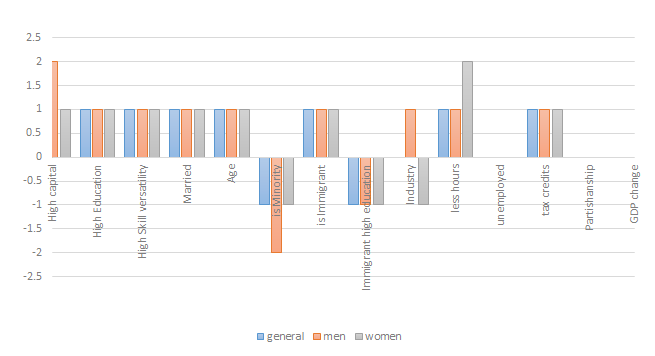
\includegraphics[width=1\linewidth]{ch-methodology/expectations.png}%
       	}%
        \caption{Hypotheses across Covariates of Interest}  
\end{figure}

These are Liquidity constraints, Demographic controls, Job Characteristics, Policy Environment and Location variables. In light of existing literature and with intuitions about where our research can bring further contributions, we frame hypotheses for their effects and underlying mechanisms. Figure 4.1 illustrates our expectations schematically, labeling coefficients by sign and relative magnitude. The scale is for graphing purposes and does not speak to actual estimates.


\subsection{Dependent Variable}

The probability of becoming an entrepreneur $p_{entry}$ is estimated for each individual as the change to self-employment in the second survey month ($t_1$) after conditioned on not being self-employed in the first one ($t_0$). The sample mean is around 0.5\%, with a slight decrease in the yearly average for the period after 2008. 



\subsection{Individual-Level Variables}

\textbf{Liquidity Constraints.} Availability of capital ($log\_income$) is measured as the natural logarithm of an individual's family income at survey time $t_0$. Higher levels of liquidity are expected to lead to a higher likelihood of self-employment $p_{entry}$, and we are interested in how this effect varies across genders. We expect positive coefficients for both men and women, and given literature, suspect men to be more responsive to family income. This assumption is based on psychological studies looking at risk-aversion across genders, with findings pointing to men engaging in activities with uncertain outcomes to a greater extent than their female counterparts\footnote{\cite{francis2015gender}}\hspace{.15em},\footnote{\cite{adams2012beyond}}. If this is true, then availability of capital might not directly translate to the desire to start a business equally across genders, with women expecting more certainty in gains.

\textbf{Education.} Educational attainment ($ed\_years$) is measured in years of schooling for both men and women. We expect this variable to have a strong positive influence on self-employment entry, as higher levels of human capital often mean better access to resources needed to start one's business. Because educational attainment is intrinsically related to field of study (which we do not observe in our data), we expect the effects of education on business entry might vary across genders, with different skills induced by an agent's course of study.

\textbf{Skill versatility.} We compute versatility ($skill\_vers$) as a binary for whether the respondent changed industry in the given year, instrumented on educational attainment. Given the literature, a higher degree of skill versatility should lead to positive effects on the self-employment rate, with differences to be analyzed across genders. If women experience more rigid labor markets, and might pursue less marketable courses of study at the same level of educational attainment, they would have less possibilities for industry change. As a result, we expect to observe a coefficient that is smaller in magnitude in their case. 

\textbf{Marriage.}  Marital status ($i.marstat$) is a categorical variable, with the differentiated labels:
\begin{enumerate}
\singlespacing
\item Married, spouse present
\item Married, spouse in armed forces
\item Married, spouse absent
\item Widowed
\item Divorced
\item Never married
\end{enumerate}

Household characteristics are expected to play a large role in one's motivations to start a business, with literature predicting both genders being positively incentivized by being married. 

\textbf{Marriage and Finances.} We compute an interaction term $mar\_income$ to test whether marriage status influences the way people value financial stability in their choice to open a business. For this purpose, a binary for marriage was created, aggregating the six categories to only two values. If marriage is indeed a positive influence on the motivation to start a business, then this interaction should have a positive effect, denoting that the more liquidity couples dispose of, the greater their likelihood of business formation. 

\textbf{Age.} We expect age to be a push factor for entry decisions, with a threshold suspected for positive effects. We fit a quadratic term for the coefficients on age, and expect to see an upside down parabola with different degrees of steepness for men and women [Figure 4.2]. According to this hypothesis, individuals are more likely to become self-employed as they are becoming older and getting closer to a certain age, after which the curve slopes downward. If confirmed by coefficient estimates, this finding could nuance the discussion of aggregate age effects. 

\begin{figure}[hbtp]
	  \centering{%
		  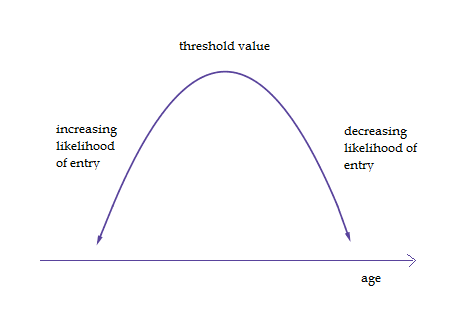
\includegraphics[width=0.6\linewidth]{ch-methodology/concavedown.png}%
    	}%
    \caption{Schematic Representation of Expected Age Effects} 
\end{figure}

\textbf{Race.} Membership to a minority group ($i.race$) is computed as a categorical variable, with coefficients indicating whether deterrents exist for particular groups. We expect being Black or Hispanic to present negative estimates for the effect on self-employment, with coefficients smaller in magnitude for the female sample. This is predicted due to more barriers associated with being a man in these racial groups. The coefficient on being Asian is expected to produce a positive effect on the self-employment rate, with interest in whether there is a differential on gender. 


\textbf{Immigration.} Immigrant status ($immigr$) is computed as a binary, with consensus in literature for positive self-employment outcomes within this category. It is nonetheless important to differentiate effects according to education, and we add an interaction term on skill level for both genders. The expectation is of a negative effect of highly-skilled immigrant status on the wish to start a business, as respondents in this group are more likely to experience a higher demand on their skills and a regulatory environment less favorable for risk taking. We are interested in whether this effect holds to the same degree for both genders, with a case to be made for different motivations for female/male immigrants. 


\subsection{Employment Characteristics}

\textbf{Industry.} We record industry at survey time $t_0$ and $t_1$, with granularity for sub-sectors coded according to NAICS guidelines. Agriculture, mining and construction were dropped from the sample, our research being interested in self-employment initiatives in manufacturing and the services sector. We use categorical variables for major industries of interest, with an interest in observing whether women see self-employment as a way to break barriers in traditionally male-dominated fields (e.g. engineering, software development or financial services).

Women are known to be underrepresented at the senior management level of companies, which only deters progress in the efforts for full gender integration\footnote{\cite{olivetti2016dp11034}}. These gaps are said to originate from ``a limited pipeline of women in entry- and mid-level roles'', which is all the more prominent in male-heavy fields\footnote{\cite{adams2012beyond}}. As a result, we wonder whether self-employment can address this issue, allowing women to break into industries by starting their own companies. If coefficients for certain industries are positive and significant for this group at survey time $t_1$, data might point to a certain barrier-breaking mechanism associated with starting one's own business. 


\textbf{Hours worked.} The $hours \geq 0$ worked by an agent at his main job are recorded at both survey times, with a binary variable for less hours following the transition from $se\_t_0 = 0$ to $se\_t_1 = 1$. We first test whether the hours worked at survey time $t_0$, conditioned $hours\_t_0 \geq 0$, contribute to the motivation to become self-employed. We are also interested whether starting a business is positively motivated by a greater degree of flexibility at work, as expressed by the coefficient on $less_hours$. 

Workers could turn to self-employment because of its associated non-monetary benefits, and not necessarily for the economic incentives. To test whether the positive effect is controlled by marriage status, we implement an interaction term for working less at $t_1$ and being married. In that sense, some married women might be more likely to adopt self-employment for the benefit of a more flexible schedule if household characteristics point to it. 

\textbf{Unemployed.} Unemployment status at $t_0$ ($unem$) becomes a measure of necessity entrepreneurship, with a positive coefficient expected for respondents who were out of work at the first survey time. The extent to which being unemployed matters for men and women has proven ambiguous, and in our research we wish to asses whether the coefficient differs in magnitude across the two groups.


\subsection{Policy Environment}

\textbf{Tax incentives.} Tax credits are measured by a binary ($tax\_credit$) indicating the existence of a tax break on new business investment in the respondent's state in the given year\footnote{The author is aware that the research framework could also use the actual corporate tax rate in a state and during the given year, a popular approach to measuring the friendliness of a policy environment to new businesses. However, the intent is to capture as much of the heterogeneity in states' different treatment of new businesses as possible, and the availability of tax credits is an approach that could provide new insights}. We are interested in how these credits incentivize business formation, and whether asymmetric effects exist for men and women. We hypothesize the coefficient is positive, and that it might vary across groups.

\textbf{Local governance.} The partisanship of the current governor ($rep\_gov$, $dem\_gov$ and $indep\_gov$) is added to asses whether men and women respond differently to political factors in deciding to pursue self-employment at a given time. Particular types of economic policies - small business loans, the willingness to implement tax breaks, programs that engage women and minorities, etc - might be more closely associated with a political ideology than the other, and could affect the incentives of people wanting to open a business. 

At the same time, a binary for party change in state level governance ($gov\_change$) has been computed, testing whether partisanship shifts provide cues for new programs and incentives. If this is the case, a positive coefficient might indicate there are new motivations associated with a change in political landscape, and there is an interest to assess whether men and women take such cues differently. 


\subsection{Macroeconomic Conditions}

\textbf{State GDP.} The coefficient on state GDP change ($gdp\_change$) from the past year measures the extent to which an individual's likelihood to start a business might respond to periods of economic upturn or downturn. This effect is complex, encompassing both a sense of real economic conditions affecting one's labor market prospects, as well as the degree to which they are assimilated by respondents into the decision to start a business.

\textbf{Education and Economic Performance.} We compute an interaction term of education and local economic prospects ($ed\_econ$), hoping to provide an intuition for an agent's demand for wage labor at a given time. As such, a negative coefficient on this interaction term would indicate that in times of economic upturn, high skill is rewarded more by wage employment. In times of downturn, there might be more incentives to join self-employment. The extent to which this effect varies for men and women speaks to both individual incentives, as well as how the U.S. labor market values work and skill level across genders. 

\textbf{State Unemployment.} The state unemployment rate ($unem\_rate$) is measure for the current year, the previous year and the change between periods. We expect a negative coefficient on unemployment, as periods of economic downturn fail to provide the necessary incentives for individuals to take the risks associated with business formation. Differences in gender might be due to different manifestations of risk aversion, as well as labor prospects in times of high unemployment. \\

We cluster errors on \textbf{metropolitan area}, and use states as controls that speak to the spatial concentration of business formation. Given that location data is categorical in nature, we expect certain states to be more influential than others, with those overlapping with historically innovative regions such as Silicon Valley or Route 128 to result in positive coefficients, while others negatively contributing to entry probability. When used to model entry rates, these variables might also capture up-and-coming entrepreneurship hubs, as opposed to established innovation clusters. 
































